\section{BÚSQUEDA DE VECINOS CERCANOS}

Uno de los métodos de búsqueda de recomendaciones más populares es el método de búsqueda de vecinos más cercanos más comunmente denominado como \text{K-Nearest Neighbors (k-NN)}. Este término es usado debido a que esta búsqueda se centra en encontrar los $k$ puntos más cercanos (o también denominados como \textit{Vecinos}) a partir de un registro de entrenamiento\parencite{10.5555/1941884}.

Se puede definir a la \textit{Búsqueda de Vecinos más cercanos} de la siguiente manera: 


\begin{definition}
    Dado un punto petición $q$ al que se le quiere conocer su clase $l$, y un conjunto de entrenamiento $X = \{ \{x_1, l_1\}\hdots\{x_n\} \}$, donde $x_j$ es el j-ésimo elemento y $l_j$ representa la etiqueta de la clase, los métodos \textit{k-NN} encuentran el subconjunto $Y = \{\{y_1, l_1\} \hdots \{y_k\} \}$ tal que $Y \in X$ y, además, $\sum^k_1d(q, y_k)$ \footnote{Representa la sumatoria de distancias entre $q$ y cada elemento $y_k \in Y$, pudiendo calcularse ya sea con distancia euclidiana, distancia de coseno o producto interno.}  se minimiza. El subconjunto $Y$ contiene los $k$ puntos en $X$ que son los más cercanos al punto petición $q$ \parencite{10.5555/1941884}.  
\end{definition}

Antes de implementar un método de \textit{Vecinos más Cercanos} es importante definir una \textit{funcion de similaridad}, según \parencite{Aggarwal2016} la más común es la \textit{Distancia de Coseno}.  Esta función de similaridad, independientemente de la elegida, cumple la función de predecir la preferencia del usuario respecto a un item que no ha evaluado. 

Una vez elegida la función de similaridad, el siguiente paso es definir el valor de $k$ que, en el punto de vista de \parencite{10.5555/1941884} es el reto más importante al usar los métodos de vecinos cercanos, debido a que un valor pequeño de $k$ incrementa la cantidad de \textit{ruido}\footnote{\textbf{Ruido}: Es definido como un error aleatorio o una varianza en una variable medida \parencite{alasadi2017review}. } en los resultados, sin embargo, si $k$ es muy grande, el vecindario podría incluir muchos puntos de diversas clases.

\begin{figure}[h!]
    \centering
    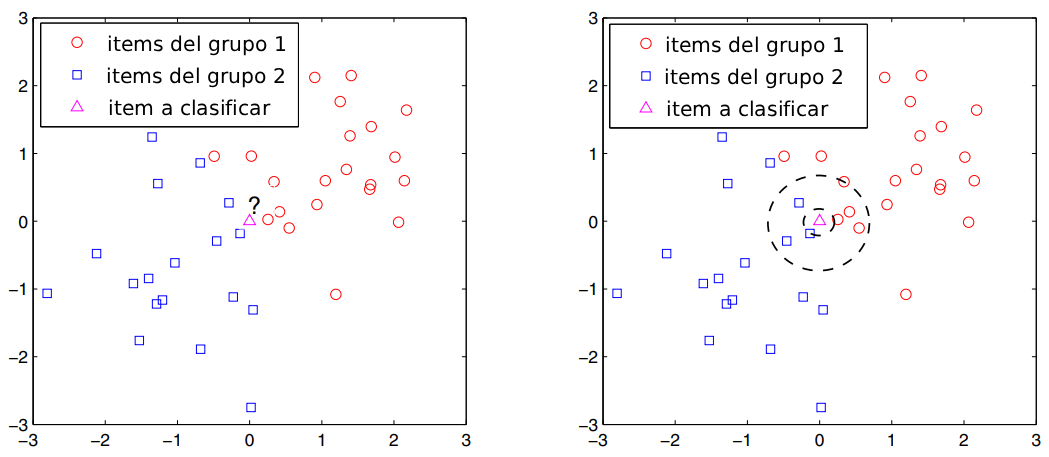
\includegraphics[width=0.8\linewidth]{NNimage.png}
    \caption{Ejemplo de Búsqueda de Vecinos Cercanos \parencite{10.5555/1941884}.}
    \label{fig:NNEjemplo}
\end{figure}

En la \Cref{fig:NNEjemplo} se muestra un ejemplo representativo de la \textit{Búsqueda de Vecinos Cercanos} que representa a dos grupos o clasificaciones, uno representado por el color rojo y otro por el color azul, y una petición representada como un triangulo. En la imágen de la izquierda se muestran los items sin clasificar, y en la imágen de la derecha se visualiza el valor de $k$ a través de círculos punteados, el circulo más pequeño representa $k = 1$ y el circulo más grande $k = 7$ 

\newpage

A través de esta descripción del funcionamiento de los algoritmos \textit{k-NN} se puede intuir que estos métodos son más simples a comparación de otros relacionados con \textit{Machine Learning} y, además, están estrechamente relacionados con el concepto de \textit{Vecindario} mencionado en la sección de \textit{Filtros Colaborativos de un Sistema de Recomendación}. Los algoritmos \textit{k-NN} suenan ideales debido a que no necesitan mantener un modelo de aprendizaje, pueden ser sencillos de implementar y, además, cuentan con las ventajas de los \textit{Filtros Colaborativos}, sin embargo, su simpleza es computacionalmente costosa.

\textit{``El reto principal relacionado al uso de este enfoque es la alta complejidad computacional. Se debe notar que el vecino más cercano de cada item $x_j \in X$ debe ser determinado, y el tiempo requerido por cada calculo es lineal al tamaño de $X$. Por lo tanto, la complejidad computacional se describe como $|\ x_j \ | \times | \ X  \ |$''} \parencite{Aggarwal2016}.

Es importante recordar que $| \ x_j \ |$ representa la \textit{dimensión} del vector $x_j$ previamente definida como $n$. Por lo tanto, la fórmula de complejidad computacional mencionada por \parencite{Aggarwal2016} expresa que el tiempo necesario para calcular los vecinos cercanos \textbf{por item} depende del tamaño del vector $x_j$ multiplicado por el tamaño total del conjunto $X$ o, en otras palabras, la cantidad total de items en el sistema. 

A pesar de este problema, el enfoque \textit{k-NN} brinda resultados muy efectivos, incluso convirtiéndose en uno de los métodos principales del \textit{enfoque colaborativo}, gracias a esto se le han hecho mejoras que aumentan su rendimiento y lo hacen viable en sistemas con cantidades masivas de información.